% Created by tikzDevice version 0.9 on 2016-01-13 23:40:06
% !TEX encoding = UTF-8 Unicode
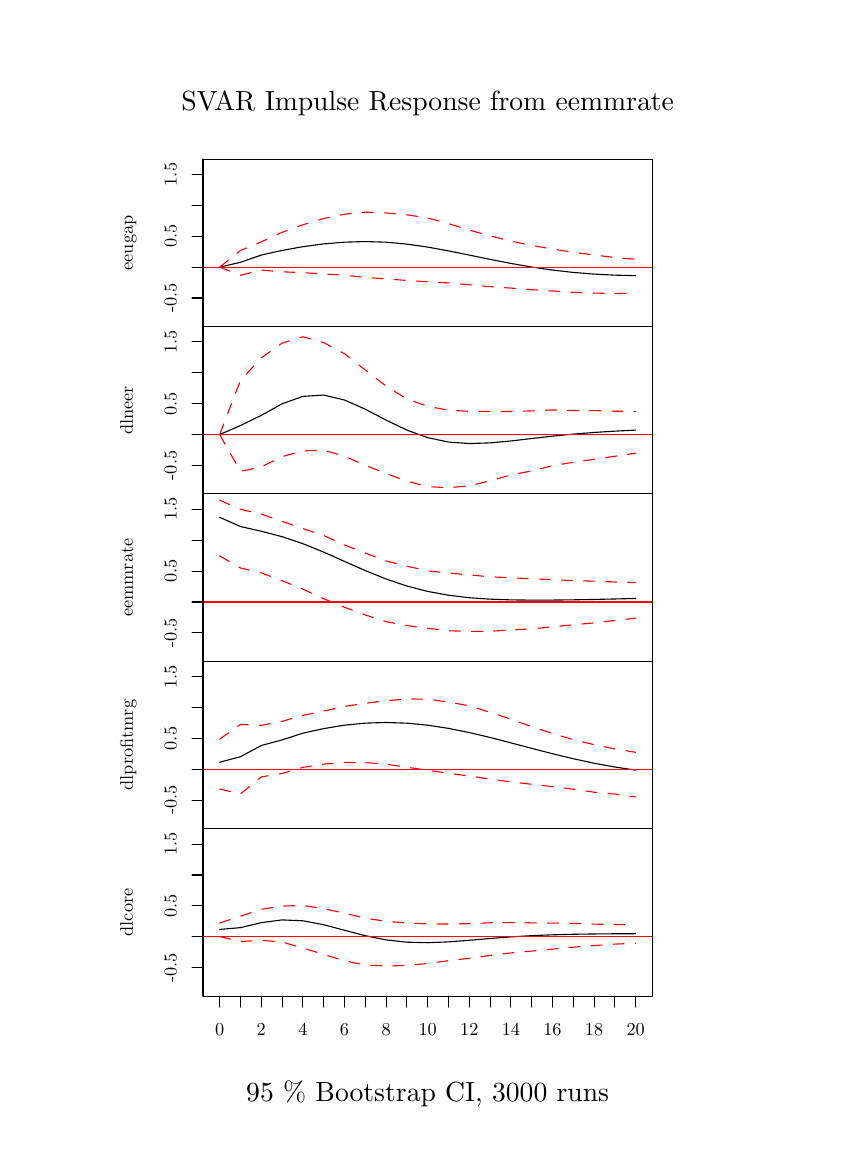
\begin{tikzpicture}[x=1pt,y=1pt]
\definecolor{fillColor}{RGB}{255,255,255}
\path[use as bounding box,fill=fillColor,fill opacity=0.00] (0,0) rectangle (289.08,397.48);
\begin{scope}
\path[clip] ( 63.36,289.48) rectangle (225.72,349.96);
\definecolor{drawColor}{RGB}{0,0,0}

\path[draw=drawColor,line width= 0.4pt,line join=round,line cap=round] ( 69.37,310.94) --
	( 76.89,312.69) --
	( 84.41,315.31) --
	( 91.92,316.99) --
	( 99.44,318.33) --
	(106.96,319.34) --
	(114.47,319.97) --
	(121.99,320.19) --
	(129.51,319.96) --
	(137.02,319.27) --
	(144.54,318.19) --
	(152.06,316.82) --
	(159.57,315.30) --
	(167.09,313.76) --
	(174.61,312.29) --
	(182.12,310.98) --
	(189.64,309.89) --
	(197.16,309.04) --
	(204.67,308.43) --
	(212.19,308.05) --
	(219.71,307.87);
\end{scope}
\begin{scope}
\path[clip] ( 31.68,289.48) rectangle (257.40,349.96);
\definecolor{drawColor}{RGB}{0,0,0}

\node[text=drawColor,anchor=base,inner sep=0pt, outer sep=0pt, scale=  0.66] at (144.54,259.38) {xy{\$}x};

\node[text=drawColor,rotate= 90.00,anchor=base,inner sep=0pt, outer sep=0pt, scale=  0.66] at ( 38.02,319.72) {eeugap};
\end{scope}
\begin{scope}
\path[clip] (  0.00,  0.00) rectangle (289.08,397.48);
\definecolor{drawColor}{RGB}{0,0,0}

\path[draw=drawColor,line width= 0.4pt,line join=round,line cap=round] ( 63.36,299.78) -- ( 63.36,349.97);

\path[draw=drawColor,line width= 0.4pt,line join=round,line cap=round] ( 63.36,299.78) -- ( 59.40,299.78);

\path[draw=drawColor,line width= 0.4pt,line join=round,line cap=round] ( 63.36,310.94) -- ( 59.40,310.94);

\path[draw=drawColor,line width= 0.4pt,line join=round,line cap=round] ( 63.36,322.10) -- ( 59.40,322.10);

\path[draw=drawColor,line width= 0.4pt,line join=round,line cap=round] ( 63.36,333.26) -- ( 59.40,333.26);

\path[draw=drawColor,line width= 0.4pt,line join=round,line cap=round] ( 63.36,344.42) -- ( 59.40,344.42);

\node[text=drawColor,rotate= 90.00,anchor=base,inner sep=0pt, outer sep=0pt, scale=  0.66] at ( 53.86,299.78) {-0.5};

\node[text=drawColor,rotate= 90.00,anchor=base,inner sep=0pt, outer sep=0pt, scale=  0.66] at ( 53.86,322.10) {0.5};

\node[text=drawColor,rotate= 90.00,anchor=base,inner sep=0pt, outer sep=0pt, scale=  0.66] at ( 53.86,344.42) {1.5};
\end{scope}
\begin{scope}
\path[clip] ( 63.36,289.48) rectangle (225.72,349.96);
\definecolor{drawColor}{RGB}{255,0,0}

\path[draw=drawColor,line width= 0.4pt,line join=round,line cap=round] ( 63.36,310.94) -- (225.72,310.94);

\path[draw=drawColor,line width= 0.4pt,dash pattern=on 4pt off 4pt ,line join=round,line cap=round] ( 69.37,310.94) --
	( 76.89,316.95) --
	( 84.41,320.07) --
	( 91.92,323.54) --
	( 99.44,326.26) --
	(106.96,328.52) --
	(114.47,330.06) --
	(121.99,330.81) --
	(129.51,330.53) --
	(137.02,329.85) --
	(144.54,328.70) --
	(152.06,326.67) --
	(159.57,324.35) --
	(167.09,322.27) --
	(174.61,320.35) --
	(182.12,318.77) --
	(189.64,317.50) --
	(197.16,316.28) --
	(204.67,315.35) --
	(212.19,314.42) --
	(219.71,313.79);

\path[draw=drawColor,line width= 0.4pt,dash pattern=on 4pt off 4pt ,line join=round,line cap=round] ( 69.37,310.94) --
	( 76.89,308.00) --
	( 84.41,309.89) --
	( 91.92,309.26) --
	( 99.44,308.96) --
	(106.96,308.46) --
	(114.47,308.02) --
	(121.99,307.25) --
	(129.51,306.68) --
	(137.02,306.14) --
	(144.54,305.63) --
	(152.06,305.25) --
	(159.57,304.58) --
	(167.09,303.90) --
	(174.61,303.37) --
	(182.12,302.82) --
	(189.64,302.31) --
	(197.16,301.83) --
	(204.67,301.58) --
	(212.19,301.41) --
	(219.71,301.50);
\end{scope}
\begin{scope}
\path[clip] (  0.00,  0.00) rectangle (289.08,397.48);
\definecolor{drawColor}{RGB}{0,0,0}

\path[draw=drawColor,line width= 0.4pt,line join=round,line cap=round] ( 63.36,289.48) --
	(225.72,289.48) --
	(225.72,349.96) --
	( 63.36,349.96) --
	( 63.36,289.48);
\end{scope}
\begin{scope}
\path[clip] ( 63.36,228.99) rectangle (225.72,289.48);
\definecolor{drawColor}{RGB}{0,0,0}

\path[draw=drawColor,line width= 0.4pt,line join=round,line cap=round] ( 69.37,250.45) --
	( 76.89,253.71) --
	( 84.41,257.37) --
	( 91.92,261.56) --
	( 99.44,264.24) --
	(106.96,264.72) --
	(114.47,262.94) --
	(121.99,259.60) --
	(129.51,255.68) --
	(137.02,252.06) --
	(144.54,249.34) --
	(152.06,247.74) --
	(159.57,247.20) --
	(167.09,247.44) --
	(174.61,248.13) --
	(182.12,249.01) --
	(189.64,249.87) --
	(197.16,250.61) --
	(204.67,251.21) --
	(212.19,251.68) --
	(219.71,252.06);
\end{scope}
\begin{scope}
\path[clip] ( 31.68,228.99) rectangle (257.40,289.48);
\definecolor{drawColor}{RGB}{0,0,0}

\node[text=drawColor,anchor=base,inner sep=0pt, outer sep=0pt, scale=  0.66] at (144.54,198.89) {xy{\$}x};

\node[text=drawColor,rotate= 90.00,anchor=base,inner sep=0pt, outer sep=0pt, scale=  0.66] at ( 38.02,259.23) {dlneer};
\end{scope}
\begin{scope}
\path[clip] (  0.00,  0.00) rectangle (289.08,397.48);
\definecolor{drawColor}{RGB}{0,0,0}

\path[draw=drawColor,line width= 0.4pt,line join=round,line cap=round] ( 63.36,239.29) -- ( 63.36,289.48);

\path[draw=drawColor,line width= 0.4pt,line join=round,line cap=round] ( 63.36,239.29) -- ( 59.40,239.29);

\path[draw=drawColor,line width= 0.4pt,line join=round,line cap=round] ( 63.36,250.45) -- ( 59.40,250.45);

\path[draw=drawColor,line width= 0.4pt,line join=round,line cap=round] ( 63.36,261.61) -- ( 59.40,261.61);

\path[draw=drawColor,line width= 0.4pt,line join=round,line cap=round] ( 63.36,272.77) -- ( 59.40,272.77);

\path[draw=drawColor,line width= 0.4pt,line join=round,line cap=round] ( 63.36,283.93) -- ( 59.40,283.93);

\node[text=drawColor,rotate= 90.00,anchor=base,inner sep=0pt, outer sep=0pt, scale=  0.66] at ( 53.86,239.29) {-0.5};

\node[text=drawColor,rotate= 90.00,anchor=base,inner sep=0pt, outer sep=0pt, scale=  0.66] at ( 53.86,261.61) {0.5};

\node[text=drawColor,rotate= 90.00,anchor=base,inner sep=0pt, outer sep=0pt, scale=  0.66] at ( 53.86,283.93) {1.5};
\end{scope}
\begin{scope}
\path[clip] ( 63.36,228.99) rectangle (225.72,289.48);
\definecolor{drawColor}{RGB}{255,0,0}

\path[draw=drawColor,line width= 0.4pt,line join=round,line cap=round] ( 63.36,250.45) -- (225.72,250.45);

\path[draw=drawColor,line width= 0.4pt,dash pattern=on 4pt off 4pt ,line join=round,line cap=round] ( 69.37,250.45) --
	( 76.89,270.02) --
	( 84.41,278.16) --
	( 91.92,283.49) --
	( 99.44,285.80) --
	(106.96,283.69) --
	(114.47,279.68) --
	(121.99,273.77) --
	(129.51,267.96) --
	(137.02,263.30) --
	(144.54,260.67) --
	(152.06,259.24) --
	(159.57,258.85) --
	(167.09,258.84) --
	(174.61,258.78) --
	(182.12,258.99) --
	(189.64,259.34) --
	(197.16,259.14) --
	(204.67,259.12) --
	(212.19,258.88) --
	(219.71,258.81);

\path[draw=drawColor,line width= 0.4pt,dash pattern=on 4pt off 4pt ,line join=round,line cap=round] ( 69.37,250.45) --
	( 76.89,237.15) --
	( 84.41,238.76) --
	( 91.92,242.45) --
	( 99.44,244.59) --
	(106.96,244.78) --
	(114.47,242.66) --
	(121.99,239.34) --
	(129.51,236.38) --
	(137.02,233.61) --
	(144.54,231.65) --
	(152.06,231.23) --
	(159.57,231.95) --
	(167.09,233.73) --
	(174.61,235.87) --
	(182.12,237.32) --
	(189.64,239.19) --
	(197.16,240.43) --
	(204.67,241.50) --
	(212.19,242.62) --
	(219.71,243.72);
\end{scope}
\begin{scope}
\path[clip] (  0.00,  0.00) rectangle (289.08,397.48);
\definecolor{drawColor}{RGB}{0,0,0}

\path[draw=drawColor,line width= 0.4pt,line join=round,line cap=round] ( 63.36,228.99) --
	(225.72,228.99) --
	(225.72,289.48) --
	( 63.36,289.48) --
	( 63.36,228.99);
\end{scope}
\begin{scope}
\path[clip] ( 63.36,168.50) rectangle (225.72,228.99);
\definecolor{drawColor}{RGB}{0,0,0}

\path[draw=drawColor,line width= 0.4pt,line join=round,line cap=round] ( 69.37,220.56) --
	( 76.89,217.21) --
	( 84.41,215.51) --
	( 91.92,213.55) --
	( 99.44,211.01) --
	(106.96,207.97) --
	(114.47,204.63) --
	(121.99,201.29) --
	(129.51,198.26) --
	(137.02,195.72) --
	(144.54,193.77) --
	(152.06,192.39) --
	(159.57,191.49) --
	(167.09,190.97) --
	(174.61,190.71) --
	(182.12,190.62) --
	(189.64,190.64) --
	(197.16,190.73) --
	(204.67,190.87) --
	(212.19,191.04) --
	(219.71,191.22);
\end{scope}
\begin{scope}
\path[clip] ( 31.68,168.50) rectangle (257.40,228.99);
\definecolor{drawColor}{RGB}{0,0,0}

\node[text=drawColor,anchor=base,inner sep=0pt, outer sep=0pt, scale=  0.66] at (144.54,138.40) {xy{\$}x};

\node[text=drawColor,rotate= 90.00,anchor=base,inner sep=0pt, outer sep=0pt, scale=  0.66] at ( 38.02,198.74) {eemmrate};
\end{scope}
\begin{scope}
\path[clip] (  0.00,  0.00) rectangle (289.08,397.48);
\definecolor{drawColor}{RGB}{0,0,0}

\path[draw=drawColor,line width= 0.4pt,line join=round,line cap=round] ( 63.36,178.80) -- ( 63.36,228.99);

\path[draw=drawColor,line width= 0.4pt,line join=round,line cap=round] ( 63.36,178.80) -- ( 59.40,178.80);

\path[draw=drawColor,line width= 0.4pt,line join=round,line cap=round] ( 63.36,189.96) -- ( 59.40,189.96);

\path[draw=drawColor,line width= 0.4pt,line join=round,line cap=round] ( 63.36,201.12) -- ( 59.40,201.12);

\path[draw=drawColor,line width= 0.4pt,line join=round,line cap=round] ( 63.36,212.28) -- ( 59.40,212.28);

\path[draw=drawColor,line width= 0.4pt,line join=round,line cap=round] ( 63.36,223.44) -- ( 59.40,223.44);

\node[text=drawColor,rotate= 90.00,anchor=base,inner sep=0pt, outer sep=0pt, scale=  0.66] at ( 53.86,178.80) {-0.5};

\node[text=drawColor,rotate= 90.00,anchor=base,inner sep=0pt, outer sep=0pt, scale=  0.66] at ( 53.86,201.12) {0.5};

\node[text=drawColor,rotate= 90.00,anchor=base,inner sep=0pt, outer sep=0pt, scale=  0.66] at ( 53.86,223.44) {1.5};
\end{scope}
\begin{scope}
\path[clip] ( 63.36,168.50) rectangle (225.72,228.99);
\definecolor{drawColor}{RGB}{255,0,0}

\path[draw=drawColor,line width= 0.4pt,line join=round,line cap=round] ( 63.36,189.96) -- (225.72,189.96);

\path[draw=drawColor,line width= 0.4pt,dash pattern=on 4pt off 4pt ,line join=round,line cap=round] ( 69.37,226.75) --
	( 76.89,223.44) --
	( 84.41,221.69) --
	( 91.92,219.12) --
	( 99.44,216.48) --
	(106.96,213.98) --
	(114.47,210.56) --
	(121.99,207.62) --
	(129.51,204.78) --
	(137.02,202.89) --
	(144.54,201.20) --
	(152.06,200.41) --
	(159.57,199.74) --
	(167.09,199.05) --
	(174.61,198.71) --
	(182.12,198.33) --
	(189.64,198.02) --
	(197.16,197.65) --
	(204.67,197.48) --
	(212.19,197.18) --
	(219.71,197.02);

\path[draw=drawColor,line width= 0.4pt,dash pattern=on 4pt off 4pt ,line join=round,line cap=round] ( 69.37,206.61) --
	( 76.89,202.23) --
	( 84.41,200.46) --
	( 91.92,197.63) --
	( 99.44,194.60) --
	(106.96,191.13) --
	(114.47,188.04) --
	(121.99,185.27) --
	(129.51,182.85) --
	(137.02,181.42) --
	(144.54,180.45) --
	(152.06,179.56) --
	(159.57,179.29) --
	(167.09,179.38) --
	(174.61,179.82) --
	(182.12,180.25) --
	(189.64,180.97) --
	(197.16,181.71) --
	(204.67,182.40) --
	(212.19,183.28) --
	(219.71,184.12);
\end{scope}
\begin{scope}
\path[clip] (  0.00,  0.00) rectangle (289.08,397.48);
\definecolor{drawColor}{RGB}{0,0,0}

\path[draw=drawColor,line width= 0.4pt,line join=round,line cap=round] ( 63.36,168.50) --
	(225.72,168.50) --
	(225.72,228.99) --
	( 63.36,228.99) --
	( 63.36,168.50);
\end{scope}
\begin{scope}
\path[clip] ( 63.36,108.01) rectangle (225.72,168.50);
\definecolor{drawColor}{RGB}{0,0,0}

\path[draw=drawColor,line width= 0.4pt,line join=round,line cap=round] ( 69.37,132.04) --
	( 76.89,134.03) --
	( 84.41,138.09) --
	( 91.92,140.10) --
	( 99.44,142.55) --
	(106.96,144.19) --
	(114.47,145.43) --
	(121.99,146.17) --
	(129.51,146.41) --
	(137.02,146.16) --
	(144.54,145.43) --
	(152.06,144.28) --
	(159.57,142.77) --
	(167.09,140.99) --
	(174.61,139.05) --
	(182.12,137.06) --
	(189.64,135.12) --
	(197.16,133.31) --
	(204.67,131.69) --
	(212.19,130.31) --
	(219.71,129.19);
\end{scope}
\begin{scope}
\path[clip] ( 31.68,108.01) rectangle (257.40,168.50);
\definecolor{drawColor}{RGB}{0,0,0}

\node[text=drawColor,anchor=base,inner sep=0pt, outer sep=0pt, scale=  0.66] at (144.54, 77.91) {xy{\$}x};

\node[text=drawColor,rotate= 90.00,anchor=base,inner sep=0pt, outer sep=0pt, scale=  0.66] at ( 38.02,138.25) {dlprofitmrg};
\end{scope}
\begin{scope}
\path[clip] (  0.00,  0.00) rectangle (289.08,397.48);
\definecolor{drawColor}{RGB}{0,0,0}

\path[draw=drawColor,line width= 0.4pt,line join=round,line cap=round] ( 63.36,118.31) -- ( 63.36,168.50);

\path[draw=drawColor,line width= 0.4pt,line join=round,line cap=round] ( 63.36,118.31) -- ( 59.40,118.31);

\path[draw=drawColor,line width= 0.4pt,line join=round,line cap=round] ( 63.36,129.47) -- ( 59.40,129.47);

\path[draw=drawColor,line width= 0.4pt,line join=round,line cap=round] ( 63.36,140.63) -- ( 59.40,140.63);

\path[draw=drawColor,line width= 0.4pt,line join=round,line cap=round] ( 63.36,151.79) -- ( 59.40,151.79);

\path[draw=drawColor,line width= 0.4pt,line join=round,line cap=round] ( 63.36,162.95) -- ( 59.40,162.95);

\node[text=drawColor,rotate= 90.00,anchor=base,inner sep=0pt, outer sep=0pt, scale=  0.66] at ( 53.86,118.31) {-0.5};

\node[text=drawColor,rotate= 90.00,anchor=base,inner sep=0pt, outer sep=0pt, scale=  0.66] at ( 53.86,140.63) {0.5};

\node[text=drawColor,rotate= 90.00,anchor=base,inner sep=0pt, outer sep=0pt, scale=  0.66] at ( 53.86,162.95) {1.5};
\end{scope}
\begin{scope}
\path[clip] ( 63.36,108.01) rectangle (225.72,168.50);
\definecolor{drawColor}{RGB}{255,0,0}

\path[draw=drawColor,line width= 0.4pt,line join=round,line cap=round] ( 63.36,129.47) -- (225.72,129.47);

\path[draw=drawColor,line width= 0.4pt,dash pattern=on 4pt off 4pt ,line join=round,line cap=round] ( 69.37,140.39) --
	( 76.89,145.69) --
	( 84.41,145.37) --
	( 91.92,146.82) --
	( 99.44,148.97) --
	(106.96,150.53) --
	(114.47,152.21) --
	(121.99,153.34) --
	(129.51,154.26) --
	(137.02,154.89) --
	(144.54,154.85) --
	(152.06,153.80) --
	(159.57,152.45) --
	(167.09,150.08) --
	(174.61,147.62) --
	(182.12,144.88) --
	(189.64,142.44) --
	(197.16,140.19) --
	(204.67,138.39) --
	(212.19,136.83) --
	(219.71,135.63);

\path[draw=drawColor,line width= 0.4pt,dash pattern=on 4pt off 4pt ,line join=round,line cap=round] ( 69.37,122.39) --
	( 76.89,120.57) --
	( 84.41,126.74) --
	( 91.92,127.98) --
	( 99.44,130.19) --
	(106.96,131.37) --
	(114.47,131.95) --
	(121.99,131.93) --
	(129.51,131.31) --
	(137.02,130.24) --
	(144.54,129.13) --
	(152.06,128.05) --
	(159.57,127.06) --
	(167.09,125.95) --
	(174.61,124.93) --
	(182.12,124.09) --
	(189.64,123.23) --
	(197.16,122.30) --
	(204.67,121.22) --
	(212.19,120.54) --
	(219.71,119.52);
\end{scope}
\begin{scope}
\path[clip] (  0.00,  0.00) rectangle (289.08,397.48);
\definecolor{drawColor}{RGB}{0,0,0}

\path[draw=drawColor,line width= 0.4pt,line join=round,line cap=round] ( 63.36,108.01) --
	(225.72,108.01) --
	(225.72,168.50) --
	( 63.36,168.50) --
	( 63.36,108.01);
\end{scope}
\begin{scope}
\path[clip] ( 63.36, 47.52) rectangle (225.72,108.01);
\definecolor{drawColor}{RGB}{0,0,0}

\path[draw=drawColor,line width= 0.4pt,line join=round,line cap=round] ( 69.37, 71.63) --
	( 76.89, 72.28) --
	( 84.41, 74.07) --
	( 91.92, 75.07) --
	( 99.44, 74.75) --
	(106.96, 73.33) --
	(114.47, 71.33) --
	(121.99, 69.36) --
	(129.51, 67.85) --
	(137.02, 67.02) --
	(144.54, 66.83) --
	(152.06, 67.13) --
	(159.57, 67.71) --
	(167.09, 68.35) --
	(174.61, 68.93) --
	(182.12, 69.38) --
	(189.64, 69.68) --
	(197.16, 69.88) --
	(204.67, 69.99) --
	(212.19, 70.06) --
	(219.71, 70.09);
\end{scope}
\begin{scope}
\path[clip] ( 31.68, 47.52) rectangle (257.40,108.01);
\definecolor{drawColor}{RGB}{0,0,0}

\node[text=drawColor,anchor=base,inner sep=0pt, outer sep=0pt, scale=  0.66] at (144.54, 17.42) {xy{\$}x};

\node[text=drawColor,rotate= 90.00,anchor=base,inner sep=0pt, outer sep=0pt, scale=  0.66] at ( 38.02, 77.76) {dlcore};
\end{scope}
\begin{scope}
\path[clip] (  0.00,  0.00) rectangle (289.08,397.48);
\definecolor{drawColor}{RGB}{0,0,0}

\path[draw=drawColor,line width= 0.4pt,line join=round,line cap=round] ( 63.36, 57.82) -- ( 63.36,108.01);

\path[draw=drawColor,line width= 0.4pt,line join=round,line cap=round] ( 63.36, 57.82) -- ( 59.40, 57.82);

\path[draw=drawColor,line width= 0.4pt,line join=round,line cap=round] ( 63.36, 68.98) -- ( 59.40, 68.98);

\path[draw=drawColor,line width= 0.4pt,line join=round,line cap=round] ( 63.36, 80.14) -- ( 59.40, 80.14);

\path[draw=drawColor,line width= 0.4pt,line join=round,line cap=round] ( 63.36, 91.30) -- ( 59.40, 91.30);

\path[draw=drawColor,line width= 0.4pt,line join=round,line cap=round] ( 63.36,102.46) -- ( 59.40,102.46);

\node[text=drawColor,rotate= 90.00,anchor=base,inner sep=0pt, outer sep=0pt, scale=  0.66] at ( 53.86, 57.82) {-0.5};

\node[text=drawColor,rotate= 90.00,anchor=base,inner sep=0pt, outer sep=0pt, scale=  0.66] at ( 53.86, 80.14) {0.5};

\node[text=drawColor,rotate= 90.00,anchor=base,inner sep=0pt, outer sep=0pt, scale=  0.66] at ( 53.86,102.46) {1.5};

\path[draw=drawColor,line width= 0.4pt,line join=round,line cap=round] ( 69.37, 47.52) -- (219.71, 47.52);

\path[draw=drawColor,line width= 0.4pt,line join=round,line cap=round] ( 69.37, 47.52) -- ( 69.37, 43.56);

\path[draw=drawColor,line width= 0.4pt,line join=round,line cap=round] ( 76.89, 47.52) -- ( 76.89, 43.56);

\path[draw=drawColor,line width= 0.4pt,line join=round,line cap=round] ( 84.41, 47.52) -- ( 84.41, 43.56);

\path[draw=drawColor,line width= 0.4pt,line join=round,line cap=round] ( 91.92, 47.52) -- ( 91.92, 43.56);

\path[draw=drawColor,line width= 0.4pt,line join=round,line cap=round] ( 99.44, 47.52) -- ( 99.44, 43.56);

\path[draw=drawColor,line width= 0.4pt,line join=round,line cap=round] (106.96, 47.52) -- (106.96, 43.56);

\path[draw=drawColor,line width= 0.4pt,line join=round,line cap=round] (114.47, 47.52) -- (114.47, 43.56);

\path[draw=drawColor,line width= 0.4pt,line join=round,line cap=round] (121.99, 47.52) -- (121.99, 43.56);

\path[draw=drawColor,line width= 0.4pt,line join=round,line cap=round] (129.51, 47.52) -- (129.51, 43.56);

\path[draw=drawColor,line width= 0.4pt,line join=round,line cap=round] (137.02, 47.52) -- (137.02, 43.56);

\path[draw=drawColor,line width= 0.4pt,line join=round,line cap=round] (144.54, 47.52) -- (144.54, 43.56);

\path[draw=drawColor,line width= 0.4pt,line join=round,line cap=round] (152.06, 47.52) -- (152.06, 43.56);

\path[draw=drawColor,line width= 0.4pt,line join=round,line cap=round] (159.57, 47.52) -- (159.57, 43.56);

\path[draw=drawColor,line width= 0.4pt,line join=round,line cap=round] (167.09, 47.52) -- (167.09, 43.56);

\path[draw=drawColor,line width= 0.4pt,line join=round,line cap=round] (174.61, 47.52) -- (174.61, 43.56);

\path[draw=drawColor,line width= 0.4pt,line join=round,line cap=round] (182.12, 47.52) -- (182.12, 43.56);

\path[draw=drawColor,line width= 0.4pt,line join=round,line cap=round] (189.64, 47.52) -- (189.64, 43.56);

\path[draw=drawColor,line width= 0.4pt,line join=round,line cap=round] (197.16, 47.52) -- (197.16, 43.56);

\path[draw=drawColor,line width= 0.4pt,line join=round,line cap=round] (204.67, 47.52) -- (204.67, 43.56);

\path[draw=drawColor,line width= 0.4pt,line join=round,line cap=round] (212.19, 47.52) -- (212.19, 43.56);

\path[draw=drawColor,line width= 0.4pt,line join=round,line cap=round] (219.71, 47.52) -- (219.71, 43.56);

\node[text=drawColor,anchor=base,inner sep=0pt, outer sep=0pt, scale=  0.66] at ( 69.37, 33.26) {0};

\node[text=drawColor,anchor=base,inner sep=0pt, outer sep=0pt, scale=  0.66] at ( 84.41, 33.26) {2};

\node[text=drawColor,anchor=base,inner sep=0pt, outer sep=0pt, scale=  0.66] at ( 99.44, 33.26) {4};

\node[text=drawColor,anchor=base,inner sep=0pt, outer sep=0pt, scale=  0.66] at (114.47, 33.26) {6};

\node[text=drawColor,anchor=base,inner sep=0pt, outer sep=0pt, scale=  0.66] at (129.51, 33.26) {8};

\node[text=drawColor,anchor=base,inner sep=0pt, outer sep=0pt, scale=  0.66] at (144.54, 33.26) {10};

\node[text=drawColor,anchor=base,inner sep=0pt, outer sep=0pt, scale=  0.66] at (159.57, 33.26) {12};

\node[text=drawColor,anchor=base,inner sep=0pt, outer sep=0pt, scale=  0.66] at (174.61, 33.26) {14};

\node[text=drawColor,anchor=base,inner sep=0pt, outer sep=0pt, scale=  0.66] at (189.64, 33.26) {16};

\node[text=drawColor,anchor=base,inner sep=0pt, outer sep=0pt, scale=  0.66] at (204.67, 33.26) {18};

\node[text=drawColor,anchor=base,inner sep=0pt, outer sep=0pt, scale=  0.66] at (219.71, 33.26) {20};

\path[draw=drawColor,line width= 0.4pt,line join=round,line cap=round] ( 63.36, 47.52) --
	(225.72, 47.52) --
	(225.72,108.01) --
	( 63.36,108.01) --
	( 63.36, 47.52);
\end{scope}
\begin{scope}
\path[clip] ( 63.36, 47.52) rectangle (225.72,108.01);
\definecolor{drawColor}{RGB}{255,0,0}

\path[draw=drawColor,line width= 0.4pt,line join=round,line cap=round] ( 63.36, 68.98) -- (225.72, 68.98);

\path[draw=drawColor,line width= 0.4pt,dash pattern=on 4pt off 4pt ,line join=round,line cap=round] ( 69.37, 73.92) --
	( 76.89, 76.41) --
	( 84.41, 78.92) --
	( 91.92, 80.07) --
	( 99.44, 80.29) --
	(106.96, 79.11) --
	(114.47, 77.52) --
	(121.99, 75.69) --
	(129.51, 74.55) --
	(137.02, 73.94) --
	(144.54, 73.63) --
	(152.06, 73.59) --
	(159.57, 73.72) --
	(167.09, 74.03) --
	(174.61, 74.13) --
	(182.12, 74.01) --
	(189.64, 73.92) --
	(197.16, 73.81) --
	(204.67, 73.55) --
	(212.19, 73.41) --
	(219.71, 73.25);

\path[draw=drawColor,line width= 0.4pt,dash pattern=on 4pt off 4pt ,line join=round,line cap=round] ( 69.37, 69.05) --
	( 76.89, 67.27) --
	( 84.41, 67.68) --
	( 91.92, 67.09) --
	( 99.44, 64.90) --
	(106.96, 62.60) --
	(114.47, 60.31) --
	(121.99, 58.77) --
	(129.51, 58.42) --
	(137.02, 58.60) --
	(144.54, 59.34) --
	(152.06, 60.33) --
	(159.57, 61.20) --
	(167.09, 62.23) --
	(174.61, 63.14) --
	(182.12, 63.81) --
	(189.64, 64.52) --
	(197.16, 65.22) --
	(204.67, 65.79) --
	(212.19, 66.33) --
	(219.71, 66.61);
\end{scope}
\begin{scope}
\path[clip] (  0.00,  0.00) rectangle (289.08,397.48);
\definecolor{drawColor}{RGB}{0,0,0}

\node[text=drawColor,anchor=base,inner sep=0pt, outer sep=0pt, scale=  1.00] at (144.54,367.39) {SVAR Impulse Response from eemmrate};

\node[text=drawColor,anchor=base,inner sep=0pt, outer sep=0pt, scale=  1.00] at (144.54,  9.50) {95 {\%} Bootstrap CI,  3000 runs};
\end{scope}
\end{tikzpicture}
